\mychapter{MCTest versões 1, 2 e 3 - Quadro de Respostas (QR)}\label{ch:experimentos_QR}

O objetivo desta parte do livro é relatar os experimentos realizados no MCTest desde a sua primeira versão (MCTest-1), os quais foram publicados como artigos científicos. Como cada nova versão do MCTest incorpora as funcionalidades das versões anteriores, em geral, é possível reproduzir os experimentos realizados nos processos de geração e correção de exames nesta versão web mais recente do MCTest (MCTest-5). Nos próximos capítulos, serão introduzidos alguns dos experimentos apresentados nos artigos, caso ainda não tenham sido abordados anteriormente. Esses exemplos serão salvos no banco de dados SQL relacionado, que estará disponível em \href{https://github.com/fzampirolli/mctest}{github.com/fzampirolli/mctest}, arquivo \verb|book/1ed-br/mctestLivro.sql|, juntamente com o conteúdo deste livro, com o intuito de enriquecer o texto e torná-lo mais interessante.

Antes de iniciar este relato de experiências, é importante mencionar que todas as publicações realizadas não teriam sido possíveis sem a participação fundamental dos colaboradores. Além disso, gostaria de destacar o apoio e contribuição dos professores da Universidade Federal do ABC (UFABC): Guiou Kobayashi, José Artur Quilici-Gonzalez e Rogério Perino de Oliveira Neves. Eles participaram do processo seletivo da Especialização em Tecnologias e Sistemas da Informação (TSI) da UFABC e colaboraram nas primeiras versões do MCTest desde 2012. Agradeço sua valiosa participação e contribuição no desenvolvimento deste projeto.

O artigo de \citeonline{2016:Kobayashi.Zampirolli.ea} detalha as três primeiras edições do TSI na modalidade de Ensino a Distância (EaD), oferecido pela UFABC, as quais foram lançadas nos anos de 2010, 2012 e 2014. O objetivo do curso é suprir a necessidade por profissionais qualificados em Tecnologia da Informação no estado de São Paulo, abrangendo localidades distantes até 200 km. O curso foi ministrado por meio de uma plataforma web. Os experimentos realizados focaram em superar desafios relacionados ao EaD, como a escalabilidade de professores, o isolamento e a autenticação dos estudantes. O projeto foi financiado pelo programa UAB (Universidade Aberta do Brasil), vinculado a CAPES (Coordenação de Aperfeiçoamento de Pessoal de Nível Superior) do governo brasileiro, permitindo que o curso fosse oferecido gratuitamente. A avaliação positiva dos cursos demonstra que uma universidade pública pode complementar a formação profissional de centenas de estudantes por meio de cursos de EaD de alta qualidade. Os resultados dos experimentos forneceram referências importantes que podem ser utilizadas em projetos futuros de EaD.

Neste primeiro capítulo de experimentos, será apresentado um resumo dos artigos que descrevem as experiências de criação de exames com QM estáticas, utilizando editores de texto como o Word ou BROffice.

%%%%%%%%%%%%%%%%%%%%%%%%%%%%%%%%%%%%%%%%%%%%%%%%%%%%%
\section{MCTest-1: versão no Matlab}
%%%%%%%%%%%%%%%%%%%%%%%%%%%%%%%%%%%%%%%%%%%%%%%%%%%%%

A primeira versão do MCTest (MCTest-1) foi utilizada no processo seletivo do TSI entre os anos de 2012 e 2017. Durante esse período, o exame era realizado no Word ou no BROffice, e a automatização era aplicada apenas na correção do exame. Para esta versão, foi publicado o seguinte artigo.

\subsection*{Artigo descrevendo a parte de visão computacional do MCTest-1}

O artigo de \citeonline{2013:Zampirolli.Quilici-Gonzalez.ea} descreve o processo de transformação de imagens capturadas dos QRs dos exames, como ilustrado na Figura \ref{fig:cap11_mctest1_folha}, em matrizes binárias reduzidas contendo as respostas às questões, juntamente com alguns elementos de controle na última coluna para as variações do exame e na última linha para atribuir pesos diferentes às questões.


\begin{figure}[!ht]
\centering
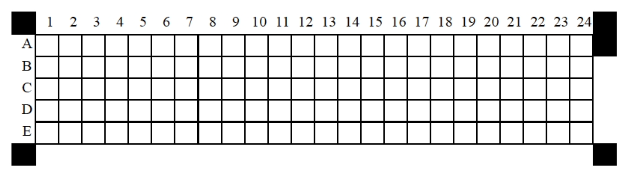
\includegraphics[width=0.8\textwidth]{cap11_mctest1_folha.png}
\caption{Recorte do PDF com o QR utilizado no MCTest-1.}
\label{fig:cap11_mctest1_folha}
\end{figure}

\subsubsection{Método}

Como o artigo foi apresentado no Workshop de Visão Computacional, o método destaca o Processamento Digital de Imagens para converter uma imagem capturada pela câmera do computador em uma matriz reduzida contendo as respostas marcadas e alguns elementos de controle adicionais.

O método foi aplicado ao problema real da correção automática de exames com QMs. Inicialmente, o usuário posiciona o QR em frente à câmera do computador para salvar a imagem no disco. Em seguida, a imagem é analisada para extrair o gabarito das variações do exame. Posteriormente, os QRs dos estudantes podem ser lidos usando o mesmo processo, e a pontuação do exame é exibida na tela e/ou salva em um arquivo.

\subsubsection{Experimentos}

Neste artigo, foi utilizada uma base de dados composta por 674 exames preenchidos por candidatos ao TSI, na oferta de 2012. Cada exame foi impresso em uma folha de papel A4 e continha 24 QMs, com cinco alternativas cada, sendo apenas uma a resposta correta. Foram preparados oito conjuntos diferentes de exames, identificados pela última coluna da Figura \ref{fig:cap11_mctest1_folha}, cada um com variações nas questões e respostas, como detalhado na Figura \ref{fig:cap11_mctest2_QR}.

O processamento dos exames foi conduzido em um MacBook Pro equipado com um processador Intel Core 2 Duo de 2,26 GHz, 2 GB de RAM e uma placa de vídeo Nvidia GeForce 9400M, que dispõe de 256 MB de memória compartilhada. Essa aquisição foi realizada por meio do projeto FAPESP \href{https://bv.fapesp.br/pt/auxilios/28430/modelagem-de-objetos-usando-morfologia-matematica-e-grafos-de-vizinhanca/}{2009/14430–1}. As capturas dos QRs preenchidos e das variações foram realizadas utilizando a câmera embutida de 2 megapixels. O processamento das imagens foi realizado por meio do MATLAB versão 2011.
%
O processamento das imagens dos exames seguiu os seguintes passos:

\begin{enumerate}
    \item Leitura das variações para cada conjunto de exames;
    \item Salvamento de uma imagem no formato TIFF contendo apenas a área do QR da variação, conforme ilustrado na Figura \ref{fig:cap11_mctest1_folha};
    \item Salvamento de uma matriz bidimensional contendo as respostas corretas para cada tipo de exame;
    \item Leitura dos QRs dos exames dos estudantes;
    \item Salvamento da imagem de cada exame em um arquivo TIFF separado;
    \item Adição dos resultados processados dos exames a um arquivo CSV.
\end{enumerate}

Os resultados dos experimentos demonstraram que o método proposto consegue corrigir automaticamente exames com QMs com alta precisão. A média de erros foi de apenas 0,2\%, representando uma precisão significativamente maior em comparação aos métodos tradicionais de correção, como a correção manual e a correção por meio de softwares comerciais testados na época.

Apesar das instruções do exame, que deixavam claro que os quadrados deveriam ser preenchidos completamente com tinta para garantir uma identificação correta, foram identificadas respostas inválidas em  6,7\% dos 674 exames (42 exames). Essas respostas foram prontamente identificadas visualmente pelo operador e a pontuação foi ajustada conforme necessário.

%%%%%%%%%%%%%%%%%%%%%%%%%%%%%%%%%%%%%%%%%%%%%%%%%%%%%
\section{MCTest-2: versão no Android}
%%%%%%%%%%%%%%%%%%%%%%%%%%%%%%%%%%%%%%%%%%%%%%%%%%%%%

\subsection*{Artigo descrevendo o MCTest-2 para dispositivos móveis}

O MCTest, Versão 2 (MCTest-2), é um aplicativo desenvolvido para dispositivos móveis, especificamente para Android, que realiza a correção automática de exames com QMs. Essa versão foi detalhado do artigo de \citeonline{2016:China.Zampirolli.ea} e é uma adaptação da primeira versão desenvolvida para computador pessoal (PC) utilizando o MATLAB. Nesta versão MCTest-2, as técnicas de processamento digital de imagens foram otimizadas para uso em dispositivos móveis, e a biblioteca \href{https://docs.opencv.org/}{OpenCV} foi empregada em substituição à ``\href{https://www.mathworks.com/products/image.html}{\textit{Toolbox de Processamento de Imagem}}'' do MATLAB.

O estudante de Iniciação Científica Rodrigo China foi responsável pelo desenvolvimento do MCTest-2, e os detalhes sobre a parte de Processamento Digital de Imagens foram publicados no Workshop de Visão Computacional \cite{2015:Zampirolli.China.ea}. Além disso, o trabalho também foi apresentado como pôster em um evento de Iniciação Científica \cite{2014:China.Zampirolli}.

\subsubsection{Método}

O artigo de \citeonline{2016:China.Zampirolli.ea} descreve o MCTest-2 desenvolvido em Java e pode ser utilizado em dispositivos com câmera embutida e sistema operacional Android, Versão 4.0 ou superior. No entanto, a resolução da câmera pode limitar o número máximo de questões e respostas no papel do exame.

O processo de utilização do aplicativo consiste em três etapas. Na primeira etapa, é possível criar um novo projeto ou carregar um projeto previamente salvo. O projeto é armazenado em uma subpasta com o nome correspondente. Na segunda etapa, os gabaritos com as respostas corretas são salvos. Esses gabaritos podem ser criados utilizando qualquer software de edição de texto. Por fim, na terceira etapa, é feita a comparação entre os exames dos estudantes e os gabaritos correspondentes. A Figura \ref{fig:cap11_mctest2_folha} demonstra o aplicativo utilizado em um gabarito impresso.

\begin{figure}[!t]
\centering
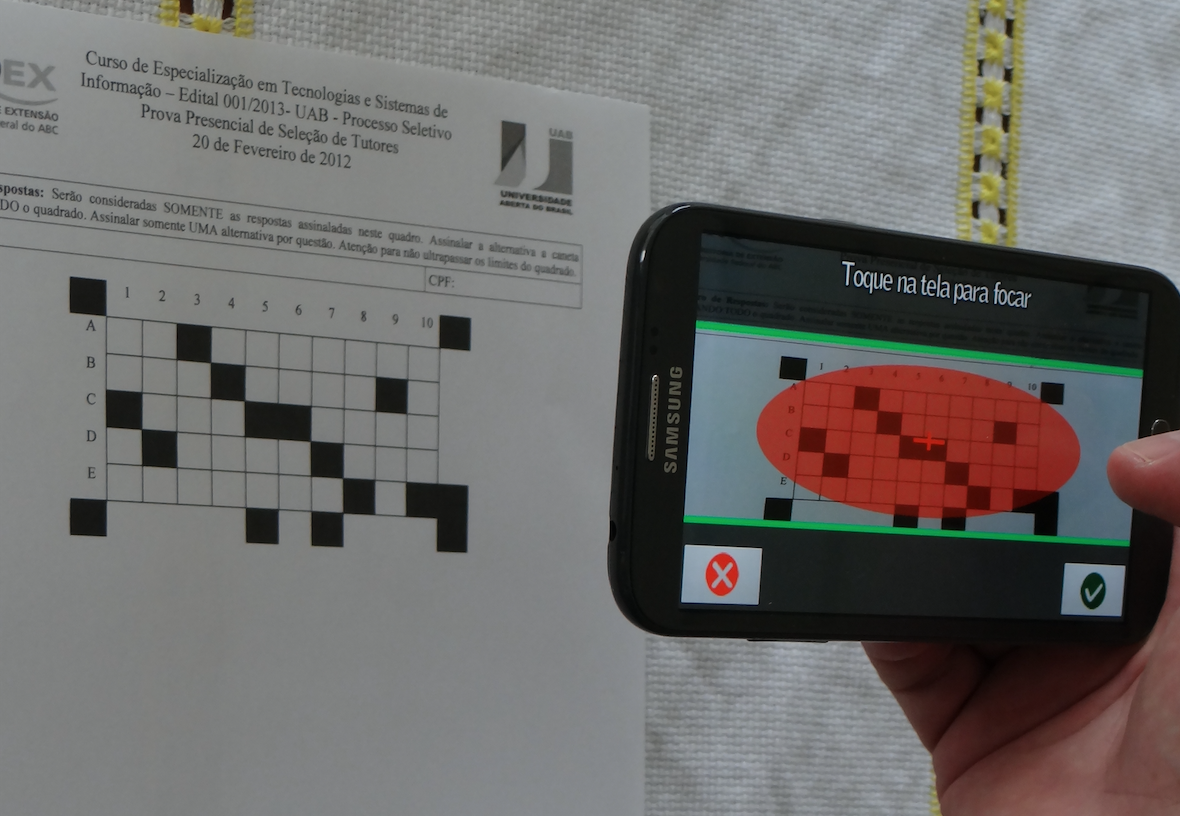
\includegraphics[width=0.8\textwidth]{cap11_mctest2_folha.png}
\caption{Demonstração da captura a partir de um gabarito impresso.}
\label{fig:cap11_mctest2_folha}
\end{figure}

A Figura \ref{fig:cap11_mctest2_QR} exibe o QR. Esse QR representa um exame com QMs com 10 questões e 5 possíveis respostas para cada questão. Uma linha e uma coluna adicionais são incluídas para armazenar informações sobre a variação de exame e a avaliação ponderada. Para identificar a variação do exame, é utilizada a coluna da direita, com os bits 0-3 indicando o número da variação em formato binário. Isso permite a criação de gabaritos de exame diferentes, com questões e respostas embaralhadas manualmente para evitar trapaças. O número de variações de exames possíveis é determinado pelo número de alternativas de resposta, e a avaliação ponderada é permitida na última linha da tabela.

\begin{figure}[!t]
\centering
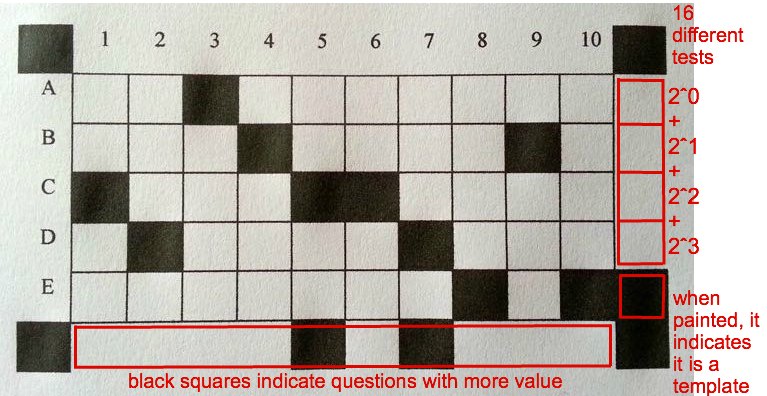
\includegraphics[width=0.7\textwidth]{cap11_mctest2_QR.jpg}
\caption{As questões marcadas na parte inferior indicam um valor ponderado atribuído a questão, as maras à direita representam diferentes gabaritos e a identificação do gabarito é a marca à direita e abaixo. Fonte: \citeonline{2016:China.Zampirolli.ea}.}
\label{fig:cap11_mctest2_QR}
\end{figure}

O QR processado e apresentado no formato CSV a seguir, gerado pelo aplicativo, contém informações sobre as respostas de dois exames. A primeira linha mostra o número de questões, respostas e quantos QRs foram processados. Em seguida, os cabeçalhos das colunas, que incluem número, ID, tipo/variação, quantidade de respostas inválidas, quantidade de respostas erradas, quantidade de respostas corretas e pontuação final. A partir da segunda linha, cada linha corresponde a um participante do exame. As colunas seguintes representam as respostas para cada uma das dez questões do exame.

Além disso, o aplicativo também oferece a opção de visualizar estatísticas por turma, conforme ilustrado na Figura \ref{fig:cap11_mctest2_estatisticas}. Esse aplicativo possui várias telas apresentadas e detalhadas no trabalho de \citeonline{2016:China.Zampirolli.ea}.


\begin{myboxCode}{corCSV}{\textbf{Conteúdo do arquivo CSV com estatísticas e as marcações realizadas.}}\vspace{3mm}
\hrule
\begin{verbatim}
10      5    2         1                                          
Numero ID Tipo Invalidas Erradas Corretas Final  Ques: 1  2  3  4  5  6  7  8  9  10
1       0    0         1       2        8   8.0   Ans: C  D  A  B  C  C  D  E  O  C
2       0    0         0       2        8   8.0   Ans: C  D  A  B  C  C  D  E  A  C
\end{verbatim}
\end{myboxCode}

\begin{figure}[!ht]
\centering
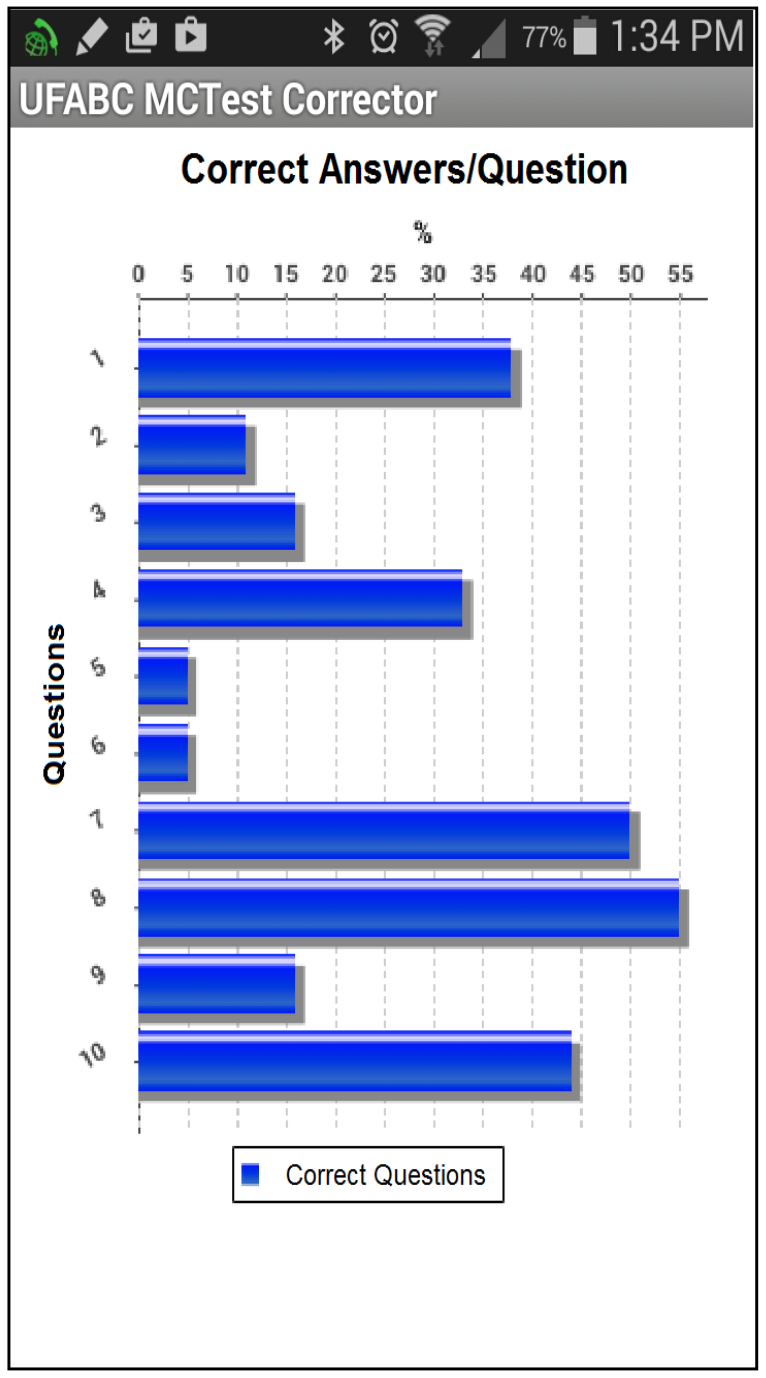
\includegraphics[width=0.3\textwidth]{cap11_mctest2_estatisticas.png}
\caption{Estatísticas sobre o número de respostas corretas em uma turma. Fonte: \citeonline{2016:China.Zampirolli.ea}.}
\label{fig:cap11_mctest2_estatisticas}
\end{figure}

\subsubsection{Experimentos}

O aplicativo foi testado em dois cenários reais, envolvendo 41 e 64 estudantes, respectivamente. Em ambos os casos, o MCTest apresentou uma precisão de 100\% quando os estudantes preencheram corretamente os QRs. O aplicativo considera os blocos preenchidos se eles contiverem pelo menos 50\% da área pintada. É importante incluir instruções claras no exame, explicando como preencher completamente o QR usando caneta preta ou lápis, a fim de evitar pontuações mais baixas.

O tempo de processamento para cada exame varia conforme o dispositivo utilizado. Contudo, mesmo em dispositivos mais acessíveis, o tempo de processamento é mais rápido do que o observado na versão anterior no computador pessoal (PC), no caso do MCTest-1.

\section{Considerações finais}

Nas diferentes versões do MCTest, existem duas abordagens para realizar os experimentos descritos. A primeira abordagem envolve fornecer as questões separadamente, como demonstrado no Capítulo \ref{ch:examesQR} - \nameref{ch:examesQR}, como utilizado na Escola Preparatória da UFABC. A segunda abordagem mais recente é incluir as questões no banco de questões do MCTest, conforme descrito no Capítulo \ref{ch:examesQM_QT} - \nameref{ch:examesQM_QT}. Além disso, nas versões mais recentes, não é mais necessário posicionar o QR diante da câmera do computador ou celular, como nas versões 1 e 2. Agora, é possível digitalizar todos os exames em um arquivo PDF, tornando o processo menos repetitivo e permitindo a correção de exames com centenas de estudantes.

A Versão 3 do MCTest (MCTest-3) foi desenvolvida em Python, utilizando o mesmo QR das versões anteriores. Nessa versão, as questões eram fornecidas separadamente e a biblioteca OpenCV era utilizada para o processamento digital de imagens. Os exames eram digitalizados em um arquivo PDF para a correção automática.

Por fim, todas as versões apresentadas neste capítulo foram registradas no INPI, conforme mencionado na Seção \ref{sec:registrosSoftware} - \nameref{sec:registrosSoftware}.

A Versão 4 do MCTest também foi desenvolvida em Python, mas agora utiliza QRs criados no \LaTeX. Além disso, as questões são geradas utilizando uma versão diferente, a 4.G (de \textit{generate}), também com o \LaTeX. Os experimentos realizados com essas versões serão apresentados no próximo capítulo.

